\lhead[\thepage]{CAPÍTULO \thechapter. \rightmark}
\rhead[CAPÍTULO \thechapter. \leftmark]{\thepage}
%======================================================================
\chapter{Números reales}
\label{nr}
\markboth{Números reales}{Números reales}
%======================================================================

%----------------------------------------------------------------------

%----------------------------------------------------------------------
En el capítulo (\ref{TC}) se vieron conjuntos de elementos que cuando tiene una característica en común se les llama conjuntos. Más explícitamente en el ejemplo (\ref{ejemplosNR}) se revisó los diferentes conjuntos de números que existen (No son los únicos). En el presente capítulo nos enfocaremos en el conjunto de los números reales, denotado por la letra $\mathbb{R}$.\\
Para representar los números reales, recurriremos al conjunto de los números irracionales ($\mathbb{I}$) y el conjunto de los números racionales ($\mathbb{Q}$), entonces la unión de estos dos conjuntos forman el conjunto de los números reales
\begin{eqnarray*}
\mathbb{R}&=&\mathbb{I}\cup \mathbb{Q} \nonumber\\
\mathbb{N}&\subset & \mathbb{Z }\subset \mathbb{Q}\subset \mathbb{R}\nonumber
\end{eqnarray*}
Mencionar que el conjunto de los números reales no es el más grande. El conjunto de los números complejos (denotado por la letra $\mathbb{C}$) es aún más grande y no se representa con una recta como reales sino con un plano de dos ejes.\\ 
\begin{figure}
	\centering
	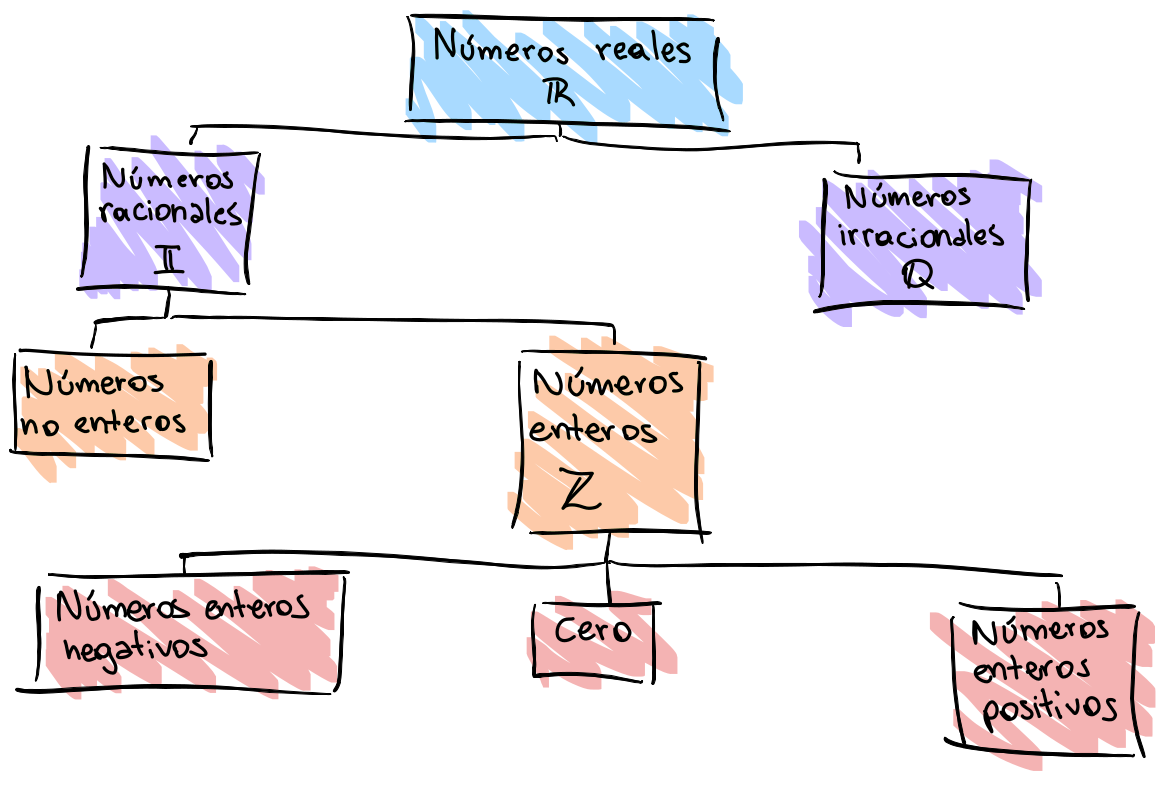
\includegraphics[scale=0.35]{esquemam.png}
	\caption[Esquema de los números reales]{Esquema de los números reales con los subconjuntos que lo conforman. }
\end{figure}
\begin{figure}
	\centering
	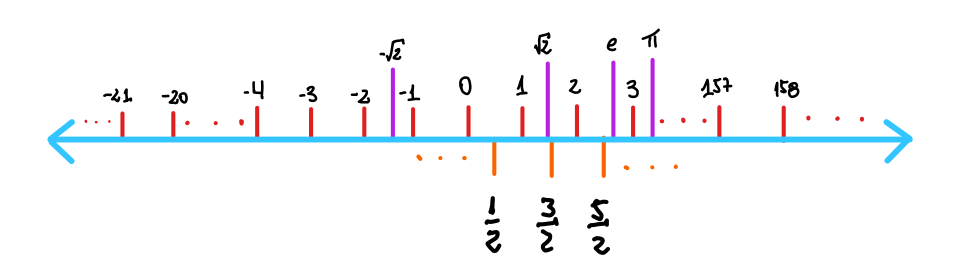
\includegraphics[scale=0.4]{rectar.png}
	\caption[Representación de la recta de los números reales]{Representación de la recta de los números reales mostrando algunos de los elementos pertenecientes a los subconjuntos que lo componen.}
	\label{rectar}
\end{figure}

\begin{myexample}
Representación de algunos elementos de los subconjuntos de los números reales
\end{myexample}

\begin{eqnarray}
\{1,3,100,263\}&\subset & \mathbb{N} \nonumber\\
\{-152,-5,0,7,670\}&\subset & \mathbb{Z} \nonumber\\
\left\{\dfrac{-3}{2},\dfrac{6}{2},\dfrac{25}{5},\dfrac{0}{9}\right\}&\subset & \mathbb{Q} \nonumber\\
\{e,\pi,\sqrt{2},\sqrt{7}\}&\subset & \mathbb{I} \nonumber\\
\left\{-10,\hspace{2px}0,\hspace{2px}\sqrt{6},\hspace{2px}2.333...,\hspace{2px}\pi,\hspace{2px}\dfrac{20}{7}\right\}&\subset & \mathbb{R} \nonumber
\end{eqnarray}

\section{Propiedades de los números reales}
\label{nr0}

El conjunto de los números reales contiene dos operaciones, una adición y una multiplicación que satisfacen las siguientes propiedades:
\subsection{Adición en los números reales}

\noindent 1) $a+(b+c)=(a+b)+c$, $\forall$ $a$, $b$, $c$ $\in \mathbb{R}$.\\

\noindent 2) $a+b=b+a$, $\forall$ $a,b\in \mathbb{R}$.\\

\noindent 3) Existe $0\in\mathbb{R}$ tal que $a+0=a$, $\forall a\in \mathbb{R}$.\\

\noindent 4) Para cada elemento $a \in \mathbb{R}$ existe un elemento $b\in\mathbb{R}$, tal que $a+b=0$. El elemento $b$ es el inverso aditivo del elemento $a$.\\

\begin{mydef}
\textbf{Sustracción.} $a-b=a+(-b)$, $\forall$ $a,b \in \mathbb{R}$ 
\end{mydef}


\subsection{Multiplicación en los números reales}
\noindent 1) $a\cdot(b\cdot c)=(a\cdot b)\cdot c$, $\forall a$, $b$, $c$ $\in \mathbb{R}$.\\

\noindent 2) $a\cdot b=b\cdot a$, $\forall$ $a$, $b$ $\in\mathbb{R}$.\\

\noindent 3) Existe $1\in\mathbb{R}$, $1\neq 0$, tal que $a\cdot 1=a$, $\forall a\in\mathbb{R}$.\\

\noindent 4) Para cada elemento $a\in\mathbb{R}$, no nulo, existe un elemento $c\in\mathbb{R}$, tal que $a\cdot c=1$. El elemento $c$ es el inverso multiplicativo de $a$ y todos los números lo tienen excepto el cero.\\

\begin{mydef}
\textbf{División.} $\dfrac{a}{b}=a\cdot b^{-1}$, $\forall a,b\in\mathbb{R}$, $b\neq 0$.
\end{mydef}

\subsection{Consecuencias de la adición y sustracción}
\label{consecu}
\noindent 1) Unicidad del 0 y del 1. Unicidad significa que existe solo un elemento dentro del conjunto, más específicamente, hay un solo elemento que cumple la acción del cero y el uno. \\

\noindent 2) Unicidad de los inversos. Tanto en la suma como en la multiplicación existe un solo inverso.\\

\noindent 3) $\forall a,b,c\in\mathbb{R}$, $a+c=b+c\Leftrightarrow a=b$. \\

\noindent 4) $\forall a,b,c\in\mathbb{R}$, $c\neq 0$, $a\cdot c=b\cdot c\Leftrightarrow a=b$. \\

\noindent 5) $a\cdot 0=0$, $\forall a\in\mathbb{R}$. \\

\noindent 6) $(-1)\cdot a=-a$, $\forall a\in\mathbb{R}$. \\

\noindent 7) $-(-a)=a$, $\forall a\in\mathbb{R}$. \\

\noindent 8) $(-a)\cdot b=a\cdot(-b)=-(a\cdot b)$; \hspace{8px} $(-a)\cdot(-b)=a\cdot b$, $\forall a,b\in\mathbb{R}$. \\

\noindent 9) Si $a\neq 0$, la ecuación $ax+b=c$ tiene solución única en $\mathbb{R}$. \\

\noindent 10) $-(a+b)=(-a)+(-b)=-a-b$, $\forall a,b\in\mathbb{R}$. \\

\noindent 11) $-(a+b)=-a-b,$ $-(-a-b)=a+b$, $\forall a,b\in\mathbb{R}$. \\

\noindent 12) $\forall a,b\in\mathbb{R}:$ $a\cdot b=0\Leftrightarrow a=0\vee b=0$. \\

\noindent 13) Si $a\neq 0$, entonces $(a^{-1})^{-1}=a$. \\

\noindent 14) Si $a,b\neq 0$, entonces $(a\cdot b)^{-1}=a^{-1}b^{-1}$. \\

\noindent 15) Si $b,d\neq 0$, $\dfrac{a}{b}=\dfrac{c}{d}\Leftrightarrow a\cdot d =b\cdot c$. \\

\noindent 16) Si $b,c\neq 0$, $\dfrac{a}{b}=\dfrac{a\cdot c}{b\cdot c}$. \\

\noindent 17) Si $c\neq 0$, $\dfrac{a}{c}\pm\dfrac{b}{c}=\dfrac{a\pm b}{c}$. \\

\noindent 18) Si $b,d \neq 0$, $\dfrac{a}{b}\cdot\dfrac{c}{d}=\dfrac{a\cdot c}{b\cdot d}$. \\

\noindent 19) Si $b,c,d\neq 0$, $\dfrac{a/b}{c/d}=\dfrac{a}{b}\cdot\dfrac{d}{c}$. \\

\noindent 20) Si $b,d\neq 0$, $\dfrac{a}{b}\pm\dfrac{c}{d}=\dfrac{a\cdot d\pm b\cdot c}{b\cdot d}$. \\
\section{Porcentajes}
De la figura (\ref{rectar}) se  pueden ver algunos elementos de los números reales son fracciones, que a su vez son números decimales. Mencionar que todo número real puede ser expresado como número decimal.
\begin{eqnarray*}
\dfrac{25}{7}=3.57142...
\end{eqnarray*}
Para algunos casos prácticos sirven estos decimales o fracciones para representar porcentajes de  alguna cantidad. Cuando se dice ``un $x$ porcentaje de algo'' se representa como
\begin{eqnarray}
\dfrac{x}{100}\cdot Cantidad
\end{eqnarray} 
Donde $x$ es el porcentaje que busco calcular de la cantidad. En algunos casos simplemente se multiplica la fracción y se multiplica directamente el número decimal por la cantidad

\begin{myexample}
Calcular el $20\%$ de $120$:
\begin{eqnarray*}
x_{20}&=&\dfrac{20}{100}\cdot 120\\
x_{20}&=&\dfrac{1}{5}\cdot 120\\
x_{20}&=&24
\end{eqnarray*}
\end{myexample}

Para otro caso que se utilizan los porcentajes, es para calcular el porcentaje de crecimiento o decrecimiento de cierta cantidad.\\

\noindent \textit{Porcentaje de aumento:}\\
\begin{eqnarray}
\dfrac{Cantidad\hspace{3px}de\hspace{3px}aumento}{Cantidad\hspace{3px}original}\times 100\%
\end{eqnarray}

\begin{eqnarray}
\dfrac{Valor\hspace{3px}final\hspace{3px}-\hspace{3px}Valor\hspace{3px}inicial}{Valor\hspace{3px}inicial}\times 100\%= \dfrac{V_{f}-V_{i}}{V_{i}}\times 100\%
\end{eqnarray}


\noindent \textit{Porcentaje de decrecimiento:}\\
\begin{eqnarray}
\dfrac{Cantidad\hspace{3px}de\hspace{3px}decrecimiento}{Cantidad\hspace{3px}original}\times 100\%
\end{eqnarray}

\begin{eqnarray}
\dfrac{Valor\hspace{3px}inicial\hspace{3px}-\hspace{3px}Valor\hspace{3px}final}{Valor\hspace{3px}inicial}\times 100\%=\dfrac{V_{i}-V_{f}}{V_{i}}\times 100\%
\label{percent1}
\end{eqnarray}


\noindent \textit{Porcentaje de transmición:}\\

\begin{eqnarray}
\dfrac{Cantidad\hspace{3px}despu\acute{e} s\hspace{3px}de\hspace{3px}Transmitirse}{Cantidad\hspace{3px}original}\times 100\%
\label{percent2}
\end{eqnarray}

\begin{myexample}
Un día por un canal entraron $150$ litros de agua, pero como estaba roto salieron solo $100$ litros, ¿Cuál es el porcentaje de transmisión del canal?\\

Sol: Primero, se identifica las cantidades que se deben reemplazar en (\ref{percent2}). 
\begin{eqnarray*}
\dfrac{100 \hspace{3px}litros}{150\hspace{3px}litros}&\times & 100\%\\
\dfrac{2}{3}&\times & 100\%\\
& 66,7\% &
\end{eqnarray*}
\end{myexample}

\begin{myexample}
El ejemplo anterior se puede resolver también con la formula de decreciemiento. Si definimos $V_{i}=150$ $litros$ y $V_{f}=100$ $litros$. 
\begin{eqnarray*}
\dfrac{V_{i}-V_{f}}{V_{i}}\times 100\% &=&\dfrac{150-100\hspace{3px}litros}{150\hspace{3px}litros}\times 100\%\\
&=& \dfrac{50\hspace{3px}litros}{150\hspace{3px}litros}\times 100\%\\
&=&\dfrac{1}{3}\times 100\%\\
&=&33,3\%
\end{eqnarray*}
\end{myexample}

Con las fórmulas de porcentaje se puede obtener diferente información desde un mismo problema según lo que uno necesite.\\
 
\section{Desigualdades}

En la figura (\ref{rectar}) se muestra la recta de los números reales, donde uno puede definir el elemento cero como el \textit{origen} y cada número, ya sea positivo o negativo, tener una distancia con respecto a ese origen. Cada número real puede representarte como un punto en esta recta que se llama \textit{coordenada}, pero usualmente solo se dice $5$ y no ``el punto $5$''.\\
Esta distancia que tienen los números permite dar un orden a los números reales, entonces si tomamos dos elementos $a$ y $b$ se puede decir las siguientes afirmaciones.\\

Si $a$ está a la izquierda de $b$, se dice que $a$ es menor que $b$ y se denota $a<b$. El otro caso es que si $a$ está a la derecha de $b$, entonces se dice que $a$ es mayor que $b$ y se denota $a>b$. Siguiendo esa lógica están los caso de menor o igual que se denota como $a\leq b$ y mayor igual $a\geq b$ que agrega la posibilidad que los elementos sean iguales. Estos cuatro elementos son los símbolos de las desigualdades.\\

Para definir las propiedades de las desigualdades se debe utilizar un subconjunto de los números reales que llamaremos $\mathbb{P}$ ($\mathbb{P}\subset\mathbb{R}$) donde sus elementos son los números positivos.\\

\noindent 1) $\forall a,b\in\mathbb{R}$, $a,b\in\mathbb{P}\Rightarrow a+b\in\mathbb{P}$ \\

\noindent 2) $\forall a,b\in\mathbb{R}$, $a,b\in\mathbb{P}\Rightarrow a\cdot b\in\mathbb{P}$ \\

\noindent Dado $a\in\mathbb{R}$, se verifica una y solo una de las alternativas:\\
\begin{eqnarray*}
a\in\mathbb{P}, \hspace{3px} a=0, \hspace{3px} -a\in\mathbb{R}
\end{eqnarray*}

\begin{mydef}
Dado $a,b\in\mathbb{R}$ se define:\\

\noindent 1) $a<b\Leftrightarrow b-a\in\mathbb{P}$.\\
\noindent 2) $a\leq b\Leftrightarrow a<b\vee a=b$. \\
\noindent 3) $a>b\Leftrightarrow b<a$. \\
\noindent 4) $a\geq b\Leftrightarrow b\leq a$. \\
\end{mydef}

\subsection{Propiedades de las desigualdades}

\noindent 1) $\forall a\in\mathbb{R}$, $a>0\Leftrightarrow a\in\mathbb{P}$ \\

\noindent 2) $a\in\mathbb{R}$,  $a<0\Leftrightarrow -a>0$ \\
\noindent 3) Para cada $a\neq 0$, $a^{2}>0$ \\
\noindent 4) Para $a,b,c\in\mathbb{R}$, 
$$\left\{\begin{array}{ll} 
a<b \\
\hspace{35px}\Rightarrow a<c\\
b<c
\end{array} \right. \\$$

\noindent 5) Para $a,b,c\in\mathbb{R}$ $a<b\Leftrightarrow a+c<b+c$\\

\noindent 6) Para $a,b,c,d\in\mathbb{R}$
$$
\left\{\begin{array}{ll}
a<b\\
\hspace{35px} \Rightarrow a+c<b+d\\
c<d
\end{array}\right. $$\\

\noindent 7) $a,b,c\in\mathbb{R}, c>0$, $a<b\Leftrightarrow a\cdot c< b\cdot c$\\

\noindent 8) $a,b,c\in\mathbb{R}, c<0$, $a<b\Leftrightarrow a\cdot c> b\cdot c$\\

\noindent 9) $a>0\Leftrightarrow a^{-1}>0$, \hspace{10px} $a<0\Leftrightarrow a^{-1}<0$

\noindent 10) $$ a\cdot b>0\Leftrightarrow \left\{ 
\begin{array}{ll}
a>0 \wedge b>0\\
\vee \\
a<0 \wedge b<0
\end{array}
\right. $$

\noindent 11) $$ a\cdot b<0 \left\{\begin{array}{ll}
a>0 \wedge b<0\\
\vee \\
a<0 \wedge b>0
\end{array} \right.$$

\noindent 12) Para $a,b>0$, $a<b\Leftrightarrow a^{-1}>b^{-1}$

\subsection{Intervalos con desigualdades}
Es momento de juntar lo visto hasta el momento de conjuntos con los conceptos de las desigualdades. Utilizaremos el paréntesis cuadrado (en algunos textos ocupan otros tipos de paréntesis) para identificar cuando un intervalo es \textit{cerrado} o \textit{abierto}.\\
\begin{eqnarray}
\left] a,b\right[ =\left\{x\in\mathbb{R}:a<x<b\right\} \label{abierto}\\
\left[ a,b\right] = \left\{x\in\mathbb{R}:a\leq x\leq b\right\}\label{cerrado} \\
\left[a,b\right[=\left\{x\in\mathbb{R}:a\leq x< b\right\}\label{abiertob} \\
\left]a,b\right]=\left\{x\in\mathbb{R}:a< x\leq b\right\} \label{abiertoa}
\end{eqnarray}
El caso (\ref{abierto}) se llama un intervalo abierto en ambos extremos o solamente abierto, esto significa que los elementos $a$ y $b$ no pertenecen al conjunto. Para el caso (\ref{cerrado}) es un conjunto cerrado, por lo que si considera a los elementos $a$ y $b$. Los casos (\ref{abiertob}) y (\ref{abiertoa}) son abiertos en un solo extremo y siguen las mismas reglas que los otros dos casos anteriores. Cuando hay un infinito en el intervalo siempre se considera abierto por ese extremo.
\begin{eqnarray}
\left]a,+\infty\right[=\{x\in\mathbb{R}:x>a\}\\
\left[a,+\infty\right[=\{x\in\mathbb{R}:x\geq a\}\\
\left]-\infty ,a\right[=\{x\in\mathbb{R}:x< a\}\\
\left]-\infty ,a\right]=\{x\in\mathbb{R}:x\leq a\}
\label{interif}
\end{eqnarray}

\section{Valor absoluto}
Así como anteriormente se mencionó que la recta permite dar orden a los números reales, también puede representar una distancia. Esta distancia que tiene un elemento dado con respecto al origen es el \textit{valor absoluto}. Como no hay distancias negativas, la distancia es la misma para un elemento $a$ como para un elemento $-a$. La notación son dos barras verticales $||$.

\begin{mydef}
\textbf{Valor absoluto}. Sea $a\in\mathbb{R}$, entonces el valor absoluto de un número se define como:\

$$ |a| \left\{\begin{array}{ll}
a, & si \hspace{6px} a\geq 0\\
-a, & si \hspace{6px} a<0 
\end{array} \hspace{6px} \right.$$
\label{absdef}
\end{mydef}

\subsection{Propiedades del valor absoluto}
\label{Propabs}
\noindent 1) $|a|\geq 0$, $\forall a\in\mathbb{R}$ \\

\noindent 2) $\forall a\in\mathbb{R}$, $|a|=0\Leftrightarrow a=0$ \\

\noindent 3) $\forall a\in\mathbb{R}$, $|-a|=|a|$ \\

\noindent 4) $\forall a,b\in\mathbb{R}$, $|a\cdot b|=|a|\cdot|b|$ \\

\noindent 5) $\forall a,b\in\mathbb{R}$, $b\neq 0$, $\left|\dfrac{a}{b}\right|=\dfrac{|a|}{|b|}$ \\

\noindent 6) $\forall a,b\in\mathbb{R}$, $|a \pm b|\leq |a|+|b|$ \\

\noindent 7) $\forall a,b\in\mathbb{R}$, $||a|-|b||\leq |a\pm b|$ \\

\noindent 8) $\forall a,b\in\mathbb{R}$, $|a|=|b|\Rightarrow a=b \vee a= -b$ \\

\noindent 9) Si $c>0$, entonces $\forall x\in\mathbb{R}$ se cumple que:\\

9.1) $|x|=c\Leftrightarrow x=c \vee x=-c$ \\

9.2) $|x|<c\Leftrightarrow -c<x<c$\\

9.3) $|x|>c\Leftrightarrow x>c \vee x<-c$
\begin{center}
	\begin{figure}[h!]
		\centering
		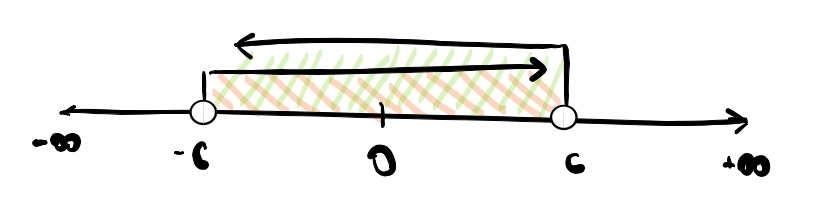
\includegraphics[scale=0.55]{abs0.png}
		\caption[Representación de un caso de valor absoluto de la propiedad 9.2]{Representación de un caso de valor absoluto de la propiedad 9.2. La zona sombreada es donde se encuentre la variable $x$ y las flechas muestran el sentido de la desigualdad particular. El resultado es la intersección de ambas condiciones.}
	\end{figure}
\end{center}
\begin{center}
	\begin{figure}[h!]
		\centering
		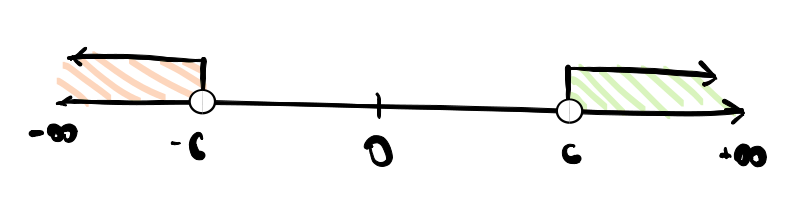
\includegraphics[scale=0.5]{abs1.png}
		\caption[Representación de un caso de valor absoluto de la propiedad 9.3]{Representación de un caso de valor absoluto de la propiedad 9.3. La zona sombreada es donde se encuentre la variable $x$ y las flechas muestran el sentido de la desigualdad particular. El resultado es la unión de ambas condiciones.}
	\end{figure}
\end{center}

\begin{myexample}
Ejercicios de valor absoluto.
\end{myexample}
\begin{eqnarray*}
&a)& |2|=2\\
&b)&|-2|=2\\
&c)&|5-7|=|-2|=2\\
&d)&|-3|-|-10|=3-(10)=-7
\end{eqnarray*}

\begin{myexample}
Encontrar el signo de la expresión $|x-6|$ para los casos cuando $a)$ $x>6$, $b)$ $x=6$ y $c)$ $x<6$
\end{myexample}
\noindent a) Primero notar que la variable toma cualquier valor mayor a $6$ y no considera al mismo número $6$. Se puede tomar cualquier número del conjunto para ver el signo del valor absoluto, por ejemplo el número $10$.\\
\begin{eqnarray}
|x-6|=|10-6|=|4|=4 \label{vaplus}
\end{eqnarray}
Entonces, de la ecuación (\ref{vaplus}) se concluye que el valor absoluto es positivo, en consecuencia $|x-6|=x-6$ para el caso cuando $x>6$.\\

\noindent b) Al igual que el caso anterior, se considera un caso particular cuando $x=6$.
\begin{eqnarray}
|x-6|=|6-6|=|0|=0
\end{eqnarray}

\noindent c) Para este último caso tomaremos un número de ejemplo, para ver el comportamiento del valor absoluto en este conjunto.
\begin{eqnarray}
|x-6|=|-10-6|=|-16|=16  \label{vapmenos}
\end{eqnarray} 
En la ecuación (\ref{vapmenos}) el resultado final es positivo por la operación del valor absoluto, pero $x-6$ es negativo por lo que se concluye que $|x-6|=-(x-6)=6-x$ cuando $x<6$.

\section{Exponentes}
\label{exponentes}
Cuando se suma varias veces una variable, para acortar la notación se escribe el número de las veces que se repite la variable y esto se multiplica por la variable, como por ejemplo $w+w+w+s+s=3w+2s$. Para el caso de la multiplicación de variables elevados a un número están las reglas de los exponentes (ya sean números enteros o fracciones) que veremos a continuación.\\

\begin{eqnarray}
x^{m}x^{n}&=&x^{m+n}\\
\left(\dfrac{x}{y}\right)^{n}&=&\dfrac{x^{n}}{y^{n}}\\
(x^{m})^{n}&=&x^{mn}\\
\dfrac{x^{m}}{x^{n}}&=&x^{m-n}\\
(xy)^{n}&=&x^{n}y^{n}
\end{eqnarray}

\subsection{Radicales}
Como se mencionó en la presentación del capítulo de exponentes, hay casos que los exponentes son fracciones y que se traducen en raíces (cuadradas, cúbicas, etc.) de la forma $\sqrt[n]{x}$, donde lo que está dentro de la raíz se llama radicando y $n$ es el índice de la raíz. Hay situaciones en que se llega a ecuaciones como $x^{2}=25$ o $y^{3}=64$ y las soluciones a estas ecuaciones se llaman \textit{raíces}, es decir, para este caso las raíces serían $5$ y el $4$ respectivamente. 
\begin{mydef}
Sea $x$ un número real y $n\geq 2$ es un número entero positivo.\\

\noindent i) Si $x>0$, entonces la raíz n-ésima principal de $\sqrt[n]{x}$  es el número r positivo tal que $x=r^{n}$.\\

\noindent ii) Si $x<0$ y n es un número entero positivo impar, entonces la raíz n-sima principal de $\sqrt[n]{x}$ es un número r negativo tal que $x=r^{n}$. Por ejemplo, la raíz cúbica está definida para cualquier número impar. \\

\noindent iii) Si $x<0$ y n es un número entero positivo par, entonces $\sqrt[n]{x}$ no es un número real. Pertenece a los números complejos ($x\in \mathbb{C}$). \\

\noindent iv) Si $x=0$, entonces $\sqrt[n]{x}=0$. \\
\end{mydef}

Las leyes que sirven para simplificar en los números radicales son las siguientes:\\
\begin{eqnarray}
&a)& (\sqrt[n]{x})^{n}=x \\
&b)& \sqrt[n]{xy}=\sqrt{x}\sqrt{y} \\
&c)& \sqrt[m]{\sqrt[n]{x}}=\sqrt[mn]{x}\\
&d)& \sqrt[n]{\dfrac{x}{y}}=\dfrac{\sqrt[n]{x}}{\sqrt[n]{y}}\\
&e)& \sqrt[n]{x^{n}}=\left\{\begin{array}{ll}
x&,\hspace{6px} si\hspace{2px} n\hspace{2px} es\hspace{2px} impar.\\
|x|& ,\hspace{6px} si\hspace{2px} n\hspace{2px} es\hspace{2px}par.
\end{array} \right.
\end{eqnarray}

\begin{myexample}
Ejercicios de exponentes
\end{myexample}
\begin{eqnarray*}
&a)& 77\cdot 77 \cdot 77\cdot 77 =77^{4}\\
&b)& 8^{-3}=\dfrac{1}{8^{3}}=\dfrac{1}{8\cdot 8\cdot 8}=\dfrac{1}{512}\\
&c)& \sqrt{2}=2^{1/2}\\
&d)& \sqrt[3]{10^{2}}=10^{2/3}\\
&e)& -5^{2}=-(5\cdot 5)=-25\\
&f)& (-5)^{2}=25\\
&g)& \sqrt{\dfrac{x^{2}}{25}}=\dfrac{\sqrt{x^{2}}}{\sqrt{25}}=\dfrac{|x|}{5}\\
&h)& \sqrt[3]{-8}=-2\\
&i)& \sqrt{256}=\sqrt{2^{8}}=2^{8/2}=2^{4}=16
\end{eqnarray*}

\subsection{Racionalización}
Se le llama racionalizar cuando ocupamos una operación matemática para quitar las raíces del numerador o denominador de una fracción. La técnica implica multiplicar por un \textit{uno} camuflado, por ejemplo:
\begin{equation*}
\dfrac{1+\sqrt{3}}{\sqrt{5}}=\dfrac{1+\sqrt{3}}{\sqrt{5}}\cdot\dfrac{\sqrt{5}}{\sqrt{5}}=\dfrac{(1+\sqrt{3})\sqrt{5}}{\sqrt{5}\cdot\sqrt{5}}=\dfrac{\sqrt{5}+\sqrt{15}}{\sqrt{5^{2}}}=\dfrac{\sqrt{5}+\sqrt{15}}{5}
\end{equation*}
Cuando el término es un factor de la forma $(\sqrt{x}\pm\sqrt{y})$ se debe multiplicar por el mismo término pero conjugado\footnote{El conjugado de una suma de números o variables consiste en cambiar el signo central entre ambos, osea que la expresión $a+b$ cambia a $a-b$, si se da el caso de $-a+b$ cambia a $-a-b$.}, es decir, el signo central es el opuesto.
$(\sqrt{x}\mp\sqrt{y})$.\\
\begin{eqnarray*}
(\sqrt{x}+\sqrt{y})(\sqrt{x}-\sqrt{y})&=& \sqrt{x}(\sqrt{x}-\sqrt{y})+\sqrt{y}(\sqrt{x}-\sqrt{y})\\
&=& (x-\sqrt{xy})+(\sqrt{yx}-y)\\
&=& x-y
\end{eqnarray*}

\begin{myexample}
Racionalizar la siguiente expresión fraccional
\end{myexample}
\begin{eqnarray*}
\dfrac{1}{\sqrt{x}+3}=\dfrac{1}{\sqrt{x}+3}\cdot \dfrac{\sqrt{x}-3}{\sqrt{x}-3}=\dfrac{\sqrt{x}-3}{x-9}
\end{eqnarray*}

Para el caso en que solo sea un término de raíz en la fracción, se debe multiplicar por el mismo termino.
\begin{eqnarray}
\dfrac{a}{\sqrt[n]{x^{k}}}\cdot\dfrac{\sqrt[n]{x^{n-k}}}{\sqrt[n]{x^{n-k}}}=\dfrac{a\sqrt[n]{x^{n-k}}}{\sqrt[n]{x^{k}}\sqrt[n]{x^{n-k}}}=\dfrac{a\sqrt[n]{x^{n-k}}}{\sqrt[n]{x^{k}\cdot x^{n-k}}}=\dfrac{a\sqrt[n]{x^{n-k}}}{\sqrt[n]{x^{k+n-k}}}=\dfrac{a\sqrt[n]{x^{n-k}}}{\sqrt[n]{x^{n}}}=\dfrac{a\sqrt[n]{x^{n-k}}}{x}
\end{eqnarray} 
Donde el número $k$ es al que está elevado el número dentro de la raíz y $n$ es la $n-$é$sima$ raíz del número.
\section{Factorización de polinomios}

\begin{mydef}
Un polinomio de grado $n$ en la variable $x$ es cualquier expresión algebraica de la forma:
\begin{eqnarray}
a_{n}x^{n}+a_{n-1}x^{n-1}+\cdots +a_{2}x^{2}+a_{1}x+a_{0}
\label{polg00}
\end{eqnarray}
con $a_{n}\neq 0$, $n$ es un número entero no negativo y $a_{i}$, $i=0,1,...,n$ son números reales.
\end{mydef}
Para los casos particulares, cuando $n=0$ es una constante, $n=1$ es un polinomio lineal, $n=2$ es un polinomio cuadratico, $n=3$ es un polinomio cúbico y para los $n\geq 4$ son polinomios de orden $n$.\\
\begin{myexample}
Sea  $5x^{4}+3x^{2}+1$ un polinomio de orden 4. Se identifican los términos desde la ecuación (\ref{polg00}) con el caso de $n=4$.
\begin{eqnarray*}
5x^{4}+3x^{2}+1&=& a_{4}x^{4}+a_{3}x^{3}+a_{2}x^{2}+a_{1}x+a_{0}x^{0}\\
&=& 5x^{4}+0x^{3}+3x^{2}+0x+1x^{0}\\
\end{eqnarray*}
Se deduce que $a_{4}=5$, $a_{3}=0$, $a_{2}=3$, $a_{1}=0$ y $a_{0}=1$.
\end{myexample}

Puede darse el caso en que hay una expresión que permite escribir un polinomio como producto de otro polinomio, esto se llama factorización. Es utilizado para simplificar resultados o separar ciertas variables. 

\begin{myexample}
Factorizar el siguiente polinomio.
\end{myexample}
\begin{eqnarray*}
6x^{4}y^{4}-4x^{2}y^{2}+10\sqrt{2}xy^{3}-2xy^{2}&=& 2xy^{2}(3x^{3}y^{2}-2x+5\sqrt{2}y-1)
\end{eqnarray*}
Lo importante en la factorización es encontrar el factor común que tienen los términos. Este factor puede ser común en todos los términos o solo en algunos.\\

\subsection{Factorización de polinomios cuadráticos}
\label{factor0}
En algunos casos es posible factorizar los polinomios cuadráticos de la forma $ax^{2}+bx+c$, donde los coeficientes $a$, $b$ y $c$ son números enteros, como 
\begin{eqnarray}
(Ax+B)(Cx+D) \label{fac0}
\end{eqnarray}
Donde $A$, $B$, $C$ y $D$ son también números enteros. Para comenzar solo consideraremos el caso en que $a=1$, entonces la ecuación queda de la forma $x^{2}+bx+c$ y los factores quedan definidos de la siguiente manera\\
\begin{eqnarray}
(x+B)(x+D) \label{fac1}
\end{eqnarray}
Si se expande la ecuación (\ref{fac1}):\\
\begin{eqnarray}
(x+B)(x+D)&=& x(x+D)+B(x+D)\nonumber\\
&=&x^{2}+xD+Bx+BD \nonumber\\
&=&x^{2}+x(D+B)+BD \label{expfac}
\end{eqnarray}
ahora se puede comparar la ecuación cuadrática término por término con la ecuación (\ref{expfac}). Se puede deducir las siguientes relaciones:
\begin{eqnarray*}
B+D=b \hspace{6px}y \hspace{6px}BD=c 
\end{eqnarray*}
\begin{myexample}
Factorizar el polinomio cuadrático de la forma $x^{2}-9x+18$
\end{myexample}
Los coeficientes son $b=-9$ y $c=18$, entonces $B+D=-9$ y $BD=18$. La segunda relación se puede escribir de diferentes formas:
\begin{eqnarray*}
1(18),\hspace{6px}2(9),\hspace{6px}3(6),\hspace{6px}-1(-18),\hspace{6px}-2(-9),\hspace{6px}o \hspace{6px}-3(-6),
\end{eqnarray*}
pero de todas las opciones anteriores solo sirve el caso en que  $B=-3$ y $D=-6$. Entonces los factores queda de la forma 
\begin{eqnarray*}
x^{2}-9x+18=(x-3)(x-6)
\end{eqnarray*}

\subsubsection{Polinomio cuadrática en caso general}
Para el caso  general donde el polinomio tiene la forma $ax^{2}+bx+c=0$ se debe aplicar la formula de ecuación cuadrática
\begin{eqnarray}
x_{\pm}=\dfrac{-b\pm\sqrt{b^{2}-4ac}}{2a}
\label{ecccuadra}
\end{eqnarray}
que se separa en dos soluciones, que son los números que componen los factores 
\begin{eqnarray}
x_{+}=\dfrac{-b+\sqrt{b^{2}-4ac}}{2a} \hspace{6px}y\hspace{6px}x_{-}=\dfrac{-b-\sqrt{b^{2}-4ac}}{2a}
\end{eqnarray}
Entonces los factores son:
\begin{eqnarray}
ax^{2}+bx+c&=&( x-x_{+})(x-x_{-})\\
&=&\left( x-\dfrac{-b+\sqrt{b^{2}-4ac}}{2a} \right) \left( x-\dfrac{-b-\sqrt{b^{2}-4ac}}{2a}\right)
\end{eqnarray}

\begin{myexample}
Resolver la ecuación cuadrática $5x^{2}+6x+1=0$
\end{myexample}
\begin{eqnarray*}
x&=&\dfrac{-6\pm\sqrt{6^{2}-4(5)(1)}}{2(5)}\\
&=&\dfrac{-6\pm\sqrt{36-20}}{10}\\
&=&\dfrac{-6\pm\sqrt{16}}{10}\\
&=&\dfrac{-6\pm 4}{10}\\
x_{+}=\dfrac{-6+ 4}{10} &y& x_{-}=\dfrac{-6- 4}{10}\\
x_{+}=\dfrac{-2}{10} &y& x_{-}=\dfrac{-10}{10}\\
x_{+}=\dfrac{-1}{5} &y& x_{-}=-1\\
\left(x+\dfrac{1}{5}\right)&\wedge &\left( x+1\right)=0
\end{eqnarray*}

Algo importante a notar en la ecuación (\ref{ecccuadra}) es el término que está bajo la raíz cuadrad al cual se le llama determinante. El término es $\sqrt{b^{2}-4ac}$ y se desprenden 3 casos posibles

\begin{itemize}
	\item Si $b^{2}-4ac>0$ la ecuación tiene soluciones distintas y reales.\\
	\item  Si $b^{2}-4ac=0$, tiene soluciones iguales y reales\\
	\item Si $b^{2}-4ac<0$ la solución pertenece a los números complejos $\mathbb{C}$.\\
\end{itemize}


\subsection{Formulas de factorización}
\label{facto}
\begin{eqnarray}
 x^{2}+2ax+a^{2}&=&(x+a)^{2} \label{fa0}\\
 x^{2}-a^{2}&=&(x+a)(x-a) \label{fa1}\\
 x^{3}-a^{3}&=&(x-a)(x^{2}+ax+a^{2})\label{fa2} \\
x^{3}+a^{3} &=& (x+a)(x^{2}-ax+a^{2}) \label{fa3}
\end{eqnarray}
La ecuación (\ref{fa0}) es un cuadrado perfecto, la ecuación (\ref{fa1}) es una diferencia de cuadrados, la ecuación (\ref{fa2}) es una diferencia de dos cubos y la ecuación (\ref{fa3}) es una suma de dos cubos. Siempre estas ecuaciones pueden cambiar las variables y no altera el resultado.

\section{Expresiones racionales}
Expandiendo el universo de posibilidades, veremos el caso de polinomios en fracciones. Aquí combinaremos lo visto en la sección anterior de polinomios con las propiedades vistas en la sección (\ref{consecu}).\\
Lo importante de esta sección es ver cuando se puede simplificar algunas expresiones, para ello, en algunos casos debemos dejar que los factores coincidan tanto en el denominador como en numerador de la fracción.\\
\begin{myexample}
Simpleficar la siguiente expresión:
\begin{eqnarray*}
\dfrac{2x^{2}-x-1}{x^{2}-1}=\dfrac{(2x+1)(x-1)}{(x+1)(x-1)}=\dfrac{2x+1}{x+1}
\end{eqnarray*}
\end{myexample}

\subsection{Mínimo común denominador (MCD)}
Al igual que en los números se busca el factor que tienen en común cada una de las fracciones. El factor se encuentra mediante la factorización de cada denominador y tomando los elementos en común que tengan. 

\begin{myexample}
Reduzca la siguiente expresión fraccional
\begin{eqnarray*}
\dfrac{x}{(x^{2}-4)}+\dfrac{1}{x^{2}+4x+4}&=& \dfrac{x}{(x-2)(x+2)}+\dfrac{1}{(x+2)^{2}}\\
&=&\dfrac{x(x+2)+(x-2)}{(x-2)(x+2)^{2}}\\
&=&\dfrac{x^{2}+2x+x-2}{(x-2)(x+2)^{2}}\\
&=&\dfrac{x^{2}+3x-2}{(x-2)(x+2)^{2}}\\
\end{eqnarray*}
\end{myexample}

\begin{myexample}
Reduzca la siguiente expresión fraccional
\begin{eqnarray*}
\dfrac{\dfrac{1}{x+h}-\dfrac{1}{x}}{h}&=&\dfrac{\dfrac{x-(x+h)}{x(x+h)}}{h}\\
&=&\dfrac{\dfrac{-h}{x(x+h)}}{h}\\
&=&\dfrac{-h}{x(x+h)}\cdot \dfrac{1}{h}\\
&=&\dfrac{-1}{x(x+h)}
\end{eqnarray*}
\end{myexample}